\section{第八周数值分析实验}
\subsection{Chebyshev多项式零点插值}
\begin{ex}
	设 $f(x)=\frac{1}{1+x^2}$, 在 $[-5,5]$ 上分别利用 $T_{11}(x), T_{15}(x), T_{21}(x)$ 的零点作为插值点,构造 $10$ 次, $14$ 次, $20 $次插值多项式 $L_{10}(x), L_{14}(x), L_{20}(x)$, 并作图表示; 此外, 作出误差曲线 $f(x)-L_{10}(x), f(x)-L_{14}(x), f(x)-L_{20}(x)$.
\end{ex}
\lstinputlisting[language=matlab]{day7/work8q1.m}
\qa 
\begin{flalign*}
	\begin{split}
		L_{10}(x)\approx & -4.7752e-6\,x^{10}+1.0795e-20\,x^9+0.00033307\,x^8-6.2457e-19\,x^7-0.0085405\,x^6\\&+1.1751e-17\,x^5+0.098309\,x^4-7.3764e-17\,x^3-0.49906\,x^2+4.8306e-17\,x+1.0.
	\end{split}&
\end{flalign*}
\begin{flalign*}
	\begin{split}
		L_{14}(x)\approx &
		-5.466e-8\,x^{14}+2.5422e-23\,x^{13}+5.179e-6\,x^{12}-0.00019734\,x^{10}+2.2204e-16\,x^9\\&+0.0038672\,x^8-0.041399\,x^6+0.23844\,x^4+5.6843e-14\,x^3-0.69456\,x^2\\&-1.1369e-13\,x+1.0.
	\end{split}&
\end{flalign*}
\begin{flalign*}
	\begin{split}
		L_{20}(x)\approx &6.7807e-11\,x^{20}+4.8908e-26\,x^{19}-8.9674e-9\,x^{18}-1.3553e-20\,x^{17}+5.0957e-7\,x^{16}\\&-1.301e-18\,x^{15}-0.000016269\,x^{14}+2.7756e-17\,x^{13}+0.00032046\,x^{12}+1.1102e-15\,x^{11}\\&-0.0040277\,x^{10}+0.032347\,x^8-1.4211e-14\,x^7-0.16239\,x^6+1.5632e-13\,x^5+0.49061\,x^4\\&-0.87049\,x^2+1.0.
	\end{split}&
\end{flalign*}
\begin{figure}[H]
	\centering
	\subfloat[Lagrange插值多项式图像]{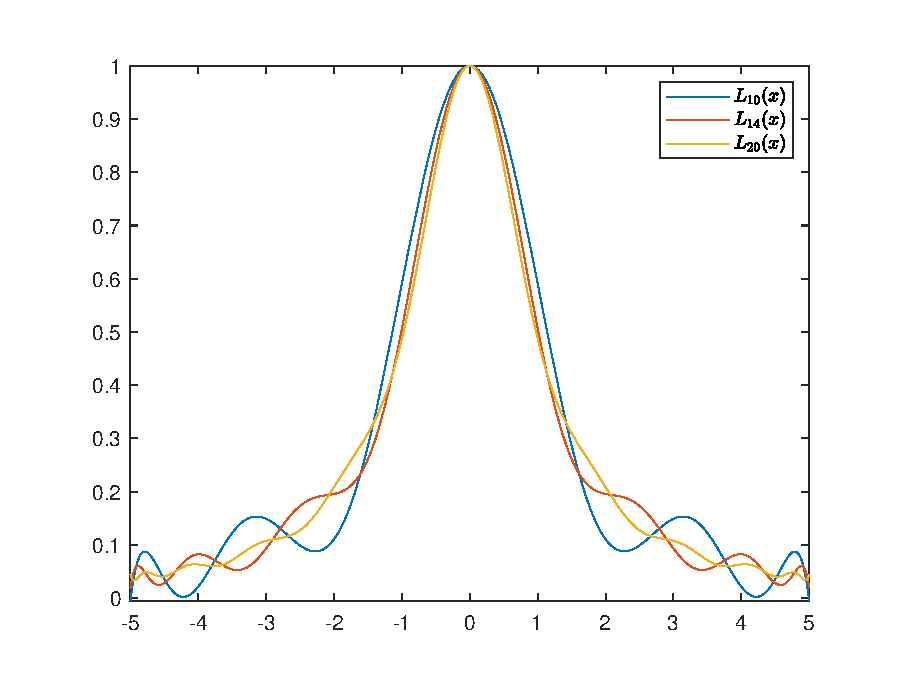
\includegraphics[width = 0.5\linewidth]{day7/q1fig1.eps}}
	\hfill
	\subfloat[误差曲线$f(x)-L_n(x)$]{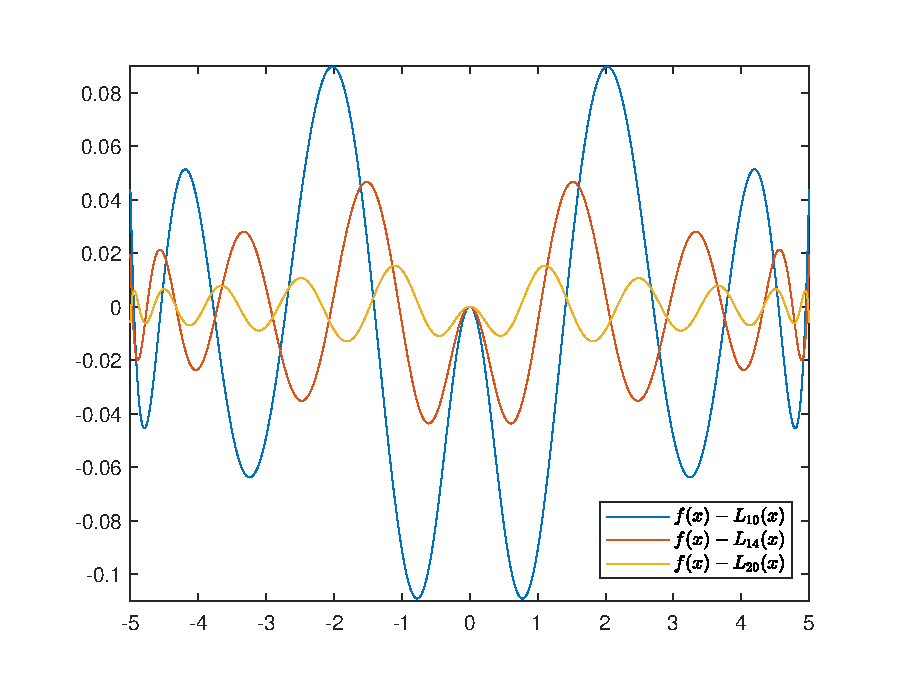
\includegraphics[width = 0.5\linewidth]{day7/q1fig2.eps}}
	\caption{结果图示}
\end{figure}
\subsection{最佳一致逼近与最佳平方逼近}
\begin{ex}
	设 $f(x)=2 x^4-3 x^3+2 x-1$, 绘制 $[0,1]$ 上的三次最佳一致逼近多项式 $P_3(x)$,二次最佳平方逼近多项式 $S_2(x)$, 伯恩斯坦多项式 $B_1(f, x), B_2(f, x), B_3(f, x)$.
\end{ex}
\subsubsection{最佳一致逼近}
\lstinputlisting[language=matlab]{day7/work8q2.m}
\qa 
\begin{flalign*}
	\begin{split}
		B_1(f,x)=x-1.
	\end{split}&
\end{flalign*}
\begin{flalign*}
	\begin{split}
		B_2(f,x)=-\frac{x^2}{2}+\frac{3\,x}{2}-1.
	\end{split}&
\end{flalign*}
\begin{flalign*}
	\begin{split}
		B_3(f,x)=\frac{2\,x^3}{9}-\frac{26\,x^2}{27}+\frac{47\,x}{27}-1.
	\end{split}&
\end{flalign*}
\begin{flalign*}
	\begin{split}
		P_3(x)=\frac{3\,x}{4}-\frac{{\left(2\,x-1\right)}^2}{4}+\frac{{\left(2\,x-1\right)}^3}{8}-\frac{41}{64}.
	\end{split}&
\end{flalign*}
\subsubsection{最佳平方逼近}
%\lstinputlisting[language=matlab]{day7/legendremap.m}
\lstinputlisting[language=matlab]{day7/work8q2s2.m}
\qa 
\begin{flalign*}
	\begin{split}
		S_2(x)=-\frac{15\,x^2}{14}+\frac{69\,x}{35}-\frac{137}{140}.
	\end{split}&
\end{flalign*}
\begin{figure}[H]
	\centering
	\subfloat[Berstein多项式及$P_3(x)$图像]{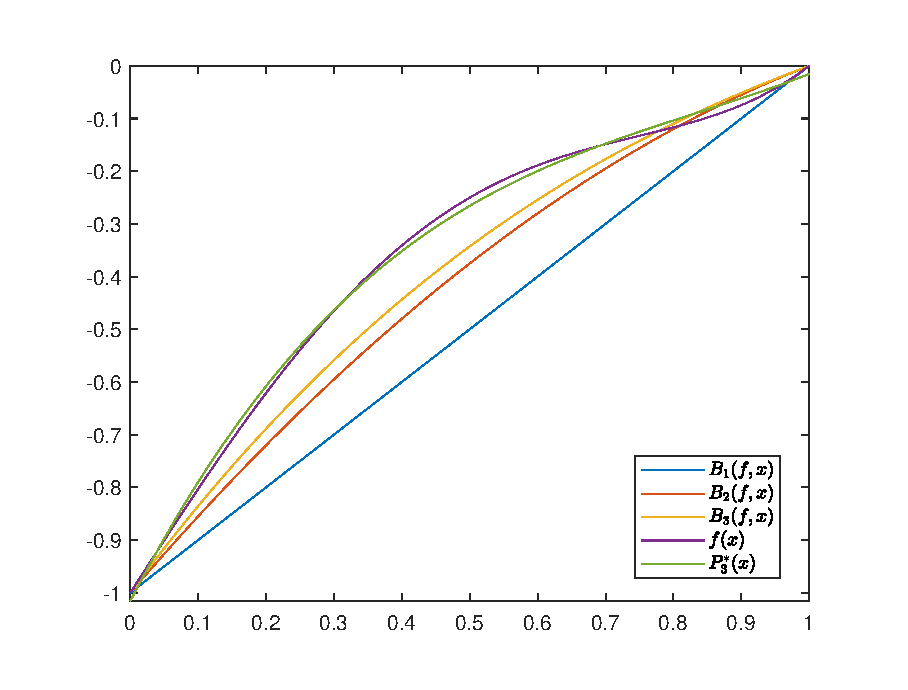
\includegraphics[width = 0.5\linewidth]{day7/q2fig1.eps}}
	\hfill
	\subfloat[二次最佳平方逼近$S_2(x)$]{\includegraphics[width = 0.5\linewidth]{day7/q2fig2.eps}}
	\caption{结果图示}
\end{figure}